%% LyX 2.2.3 created this file.  For more info, see http://www.lyx.org/.
%% Do not edit unless you really know what you are doing.
\documentclass[ruled]{article}
\usepackage{courier}
\usepackage[T1]{fontenc}
\usepackage[latin9]{inputenc}
\usepackage[letterpaper]{geometry}
\geometry{verbose}
\usepackage{color}
\usepackage{url}
\usepackage{algorithm2e}
\usepackage{amsmath}
\usepackage{amssymb}
\usepackage{titlesec}
%\newcommand{\sectionbreak}{\clearpage}
\usepackage{graphicx}
\usepackage[export]{adjustbox}
\graphicspath{ {./images/} }
\usepackage{listings}
\usepackage{pdfpages}
\usepackage[unicode=true,
 bookmarks=false,
 breaklinks=false,pdfborder={0 0 1},backref=section,colorlinks=true]
 {hyperref}

\makeatletter

%%%%%%%%%%%%%%%%%%%%%%%%%%%%%% LyX specific LaTeX commands.
\providecommand{\LyX}{\texorpdfstring%
  {L\kern-.1667em\lower.25em\hbox{Y}\kern-.125emX\@}
  {LyX}}
%% Special footnote code from the package 'stblftnt.sty'
%% Author: Robin Fairbairns -- Last revised Dec 13 1996
\let\SF@@footnote\footnote
\def\footnote{\ifx\protect\@typeset@protect
    \expandafter\SF@@footnote
  \else
    \expandafter\SF@gobble@opt
  \fi
}
\expandafter\def\csname SF@gobble@opt \endcsname{\@ifnextchar[%]
  \SF@gobble@twobracket
  \@gobble
}
\edef\SF@gobble@opt{\noexpand\protect
  \expandafter\noexpand\csname SF@gobble@opt \endcsname}
\def\SF@gobble@twobracket[#1]#2{}

\@ifundefined{date}{}{\date{}}
%%%%%%%%%%%%%%%%%%%%%%%%%%%%%% User specified LaTeX commands.
\definecolor{mygreen}{rgb}{0,0.6,0}
\definecolor{mygray}{rgb}{0.5,0.5,0.5}
\definecolor{mymauve}{rgb}{0.58,0,0.82}

\makeatother

\usepackage{listings}
\lstset{backgroundcolor={\color{white}},
basicstyle={\footnotesize\ttfamily},
breakatwhitespace=false,
breaklines=true,
captionpos=b,
commentstyle={\color{mygreen}},
deletekeywords={...},
escapeinside={\%*}{*)},
extendedchars=true,
frame=shadowbox,
keepspaces=true,
keywordstyle={\color{blue}},
language=Python,
morekeywords={*,...},
numbers=none,
numbersep=5pt,
numberstyle={\tiny\color{mygray}},
rulecolor={\color{black}},
showspaces=false,
showstringspaces=false,
showtabs=false,
stepnumber=1,
stringstyle={\color{mymauve}},
tabsize=2}

 
\begin{document}

\global\long\def\reals{\mathbf{R}}
 \global\long\def\integers{\mathbf{Z}}
\global\long\def\naturals{\mathbf{N}}
 \global\long\def\rationals{\mathbf{Q}}
\global\long\def\ca{\mathcal{A}}
\global\long\def\cb{\mathcal{B}}
 \global\long\def\cc{\mathcal{C}}
 \global\long\def\cd{\mathcal{D}}
\global\long\def\ce{\mathcal{E}}
\global\long\def\cf{\mathcal{F}}
\global\long\def\cg{\mathcal{G}}
\global\long\def\ch{\mathcal{H}}
\global\long\def\ci{\mathcal{I}}
\global\long\def\cj{\mathcal{J}}
\global\long\def\ck{\mathcal{K}}
\global\long\def\cl{\mathcal{L}}
\global\long\def\cm{\mathcal{M}}
\global\long\def\cn{\mathcal{N}}
\global\long\def\co{\mathcal{O}}
\global\long\def\cp{\mathcal{P}}
\global\long\def\cq{\mathcal{Q}}
\global\long\def\calr{\mathcal{R}}
\global\long\def\cs{\mathcal{S}}
\global\long\def\ct{\mathcal{T}}
\global\long\def\cu{\mathcal{U}}
\global\long\def\cv{\mathcal{V}}
\global\long\def\cw{\mathcal{W}}
\global\long\def\cx{\mathcal{X}}
\global\long\def\cy{\mathcal{Y}}
\global\long\def\cz{\mathcal{Z}}
\global\long\def\ind#1{1(#1)}
\global\long\def\pr{\mathbb{P}}

\global\long\def\ex{\mathbb{E}}
\global\long\def\var{\textrm{Var}}
\global\long\def\cov{\textrm{Cov}}
\global\long\def\sgn{\textrm{sgn}}
\global\long\def\sign{\textrm{sign}}
\global\long\def\kl{\textrm{KL}}
\global\long\def\law{\mathcal{L}}
\global\long\def\eps{\varepsilon}
\global\long\def\convd{\stackrel{d}{\to}}
\global\long\def\eqd{\stackrel{d}{=}}
\global\long\def\del{\nabla}
\global\long\def\loss{\ell}
\global\long\def\tr{\operatorname{tr}}
\global\long\def\trace{\operatorname{trace}}
\global\long\def\diag{\text{diag}}
\global\long\def\rank{\text{rank}}
\global\long\def\linspan{\text{span}}
\global\long\def\proj{\text{Proj}}
\global\long\def\argmax{\operatornamewithlimits{arg\, max}}
\global\long\def\argmin{\operatornamewithlimits{arg\, min}}
\global\long\def\bfx{\mathbf{x}}
\global\long\def\bfy{\mathbf{y}}
\global\long\def\bfl{\mathbf{\lambda}}
\global\long\def\bfm{\mathbf{\mu}}
\global\long\def\calL{\mathcal{L}}
\global\long\def\vw{\boldsymbol{w}}
\global\long\def\vx{\boldsymbol{x}}
\global\long\def\vxi{\boldsymbol{\xi}}
\global\long\def\valpha{\boldsymbol{\alpha}}
\global\long\def\vbeta{\boldsymbol{\beta}}
\global\long\def\vsigma{\boldsymbol{\sigma}}
\global\long\def\vmu{\boldsymbol{\mu}}
\global\long\def\vtheta{\boldsymbol{\theta}}
\global\long\def\vd{\boldsymbol{d}}
\global\long\def\vs{\boldsymbol{s}}
\global\long\def\vt{\boldsymbol{t}}
\global\long\def\vh{\boldsymbol{h}}
\global\long\def\ve{\boldsymbol{e}}
\global\long\def\vf{\boldsymbol{f}}
\global\long\def\vg{\boldsymbol{g}}
\global\long\def\vz{\boldsymbol{z}}
\global\long\def\vk{\boldsymbol{k}}
\global\long\def\va{\boldsymbol{a}}
\global\long\def\vb{\boldsymbol{b}}
\global\long\def\vv{\boldsymbol{v}}
\global\long\def\vy{\boldsymbol{y}}


\title{Machine Learning and Computational Statistics\\
Multiclass}
\author{Nhung Le}

\maketitle
\textbf{Intro}: This document consists of concepts and exercises related to Multiclass. This document discusses two main approaches One-vs-all and linear multiclass predictor.\\ 

\section{Key Concepts } 

\begin{enumerate}
\item One-vs-All
Our approach will assume we have a binary base classifier that returns a score, and we will predict the class that has the highest score.
	\begin{enumerate}
				\item pseudocode for one-vs-all (as shown in the Linear Binary Classifier Review) 
				\item Examples where one-vs-all fail: when it is too computational expensive (e.g., too many classes, a large time amount required to train one class of $n$ classes.
				

	\end{enumerate}

\item Multiclass predictor: 
Our approach is to reframe multiclass learning such that rather than using a score function for each class, we use one function $h(x, y)$ that gives a compatible score between input $x$ and output $y$. 

	\begin{enumerate}
	       \item Reframed multiclass hypothesis space: 
	        			\begin{enumerate}
	        			     \item General [discrete] output space: $Y$
	        			     \item Base hypothesis space $\ch = \{ h:\cx\times\cy\rightarrow\reals\}$ for $h(x, y)$ gives compatible score between input $x$ and output $y$
	        			     \item Multiclass hypothesis space $\cf=\left\{ f(x)=\argmax_{y\in\cy}h(x,y)\mid h\in\ch\right\} $.
	        			     \item Final prediction function is an $ f\in\cf $. Each $ f\in\cf $ has an underlying compatibility score function $h \in \ch$. 
	        			\end{enumerate}
	        \item \textbf{Compatible score}: Given class-specific score functions $h_1, h_2, \cdots, h_k$, we could define compatible score function as: $h(x, i) = h_i(x), i = 1, \cdots, k$
	        
	        \item Reframed learning in a multiclass hypothesis space: 
	                  \begin{enumerate}
	                  	 \item \textbf{Margin} of the compatibility score
function $h$ on the $i$th example $(x_{i},y_{i})$ for class $y$
\[
m_{i,y}(h)=h(x_{i},y_{i})-h(x_{i},y).
\]
						\item Two versions of Hinge Loss: 
						\begin{enumerate}
						\item Loss on an individual example $\left(x_{i},y_{i}\right)$
\[
\ell_{1}(h,(x_{i},y_{i}))=\max_{y\in\cy-\left\{ y_{i}\right\} }\left(\max\left[0,\Delta(y_{i},y)-m_{i,y}(h)\right]\right).
\] 
\item The generalized
hinge loss
\[
\ell_{2}(h,(x_{i,}y_{i}))=\max_{y\in\cy}\left[\Delta\left(y_{i},y\right)+h(x_{i},y)-h(x_{i},y_{i})\right].
\]
				   \item  if $\Delta(y,y)=0$ for all $y\in\cy$, then $\ell_{2}\left(h,\left(x_{i},y_{i}\right)\right)=\text{\ensuremath{\ell}}_{1}(h,\left(x_{i},y_{i}\right))$.
{[}Hint: Note that $\max_{y\in\cy}\phi(y)=\max\left(\phi(y_{i}),\max_{y\in\cy-\left\{ y_{i}\right\} }\phi(y_{i})\right)$.{]}\\
					\end{enumerate}						 
					 
                    \item  Non-negative class-sensitive
loss function $\Delta:\cy\times\ca\to[0,\infty)$

				\item Class-sensitive
feature mapping $\Psi:\cx\times\cy\to\reals^{d}$
				\item Linear class-sensitive score function: 
				\[
				h(x, y) = \left\langle w,\Psi(x,y)\right\rangle 
				\]
				\item Prediction
function $f:\cx\to\cy$
\[
f_{w}(x)=\argmax_{y\in\cy}\left\langle w,\Psi(x,y)\right\rangle 
\]
				\item Training data $(x_{1},y_{1}),\ldots,(x_{n},y_{n})\in\cx\times\cy$
			   \item  $J(w)$ be the $\ell_{2}$-regularized empirical risk function for the multiclass hinge loss for some $\lambda>0$.
\[
J(w)=\lambda\|w\|^{2}+\frac{1}{n}\sum_{i=1}^{n}\max_{y\in\cy}\left[\Delta\left(y_{i},y\right)+\left\langle w,\Psi(x_{i},y)-\Psi(x_{i},y_{i})\right\rangle \right],
\]

	                  \end{enumerate}
	\end{enumerate}

\item \href{https://davidrosenberg.github.io/mlcourse/ConceptChecks/7-Lec-Check_sol.pdf}{Multiclass Concept Check}
\item Map a set of linear score functions onto a single linear class-sensitive score function using a class-sensitive feature map. Give some intuition for the value of this feature map (based on features related to the target classes).
			\includepdf[scale=0.5, pages=29,pagecommand= {}, fitpaper=true,width=\textwidth]{09b-multiclass}
			
\includepdf[scale=0.5, pages=9,pagecommand= {}, fitpaper=true,width=\textwidth]{09b-multiclass}



%\includepdf[pages=28-29,pagecommand={},width=\textwidth]{08a-bayesian-regression}

\end{enumerate}
\section{Implementation} 
\subsection{Onv-vs-All Classifier} 
\begin{enumerate}
\item We have a BaseEstimator from sklearn (e.g., SVM Linear SVC) 
\item Fit one classifier for each class, knowing that self.estimators[$i$] should be fit on class i vs rest. The key here is $y_{onevsall} = 1$ when y = the class.
\item Decision function returns the score of each input for each class. 
\item Prediction function return the class with highest score.
\end{enumerate}
\subsection{Linear Multiclass SVM}
\begin{enumerate}
\item Set-up featureMap 
\item Define the Stochastic gradient descent 
\begin{enumerate}
\item Objective function for some $\lambda>0$.
\[
J(w)=\lambda\|w\|^{2}+\frac{1}{n}\sum_{i=1}^{n}\max_{y\in\cy}\left[\Delta\left(y_{i},y\right)+\left\langle w,\Psi(x_{i},y)-\Psi(x_{i},y_{i})\right\rangle \right]
\]
\item $J(w)$ is convex so it has a subgradient at every point. For $\hat{y_i} = \max_{y\in\cy} [\Delta(y_{i}, y) + \langle w,  \Psi(x_i - y) - \Psi(x_i - y_i)\rangle ]$
\[
g = 2 \lambda w + \frac{1}{n} \sum_{i=1}^{n} (\Psi(x_{i}, \hat{y_i})-\Psi(x_{i},y_{i}))
\]
\item Stochastic subgradient based on the point $(x_i, y_i)$
\[
g = 2 \lambda w + (\Psi(x_{i}, \hat{y_i})-\Psi(x_{i},y_{i}))
\]
\item Minibatch subgradient based on the point $(x_i, y_i), \cdots, (x_{i+m}, y_{i+m})$
\[
g = 2 \lambda w + \frac{1}{m} \sum_{j=i}^{i + m -1} (\Psi(x_{j}, \hat{y})-\Psi(x_{j},y_{j}))
\]
\end{enumerate}

\item Fit
\item Decision function returns the score of each input for each class.
\item Predict function returns the class with the highest score.
\end{enumerate}

\end{document}
